%\documentclass[12pt,mathserif,dvipdfmx,aspectratio=32]{beamer}
\documentclass[12pt,dvipdfmx,mathserif,uplatex,aspectratio=32]{beamer}
%\usepackage[dvipdfmx]{graphicx}
\usepackage{atbegshi}
\AtBeginShipoutFirst{\special{pdf:tounicode EUC-UCS2}}
%\AtBeginShipoutFirst{\special{pdf:tounicode 90ms-RKSJ-UCS2}}
\usepackage{minijs}
%\usepackage{oft}
\renewcommand{\kanjifamilydefault}{\gtdefault}
\usetheme{default}
%\usetheme{Antibes}
%\usecolortheme{albatross}
\setbeamertemplate{navigation symbols}{}
\setbeamercolor{frametitle}{fg=blue}
\setbeamercolor{title}{fg=black}
\setbeamercolor{table}{fg=black}
\setbeamersize{text margin right=0.5cm}
\setbeamersize{text margin left=0.5cm}
%\setbeamerfont{euler}
%\usepackage{eulervm}
\usepackage{euler}
\usepackage{multicol}
\usepackage{subfigure}

%%
%% プリアンブルに記述
%% Figure 環境中で Table 環境の見出しを表示・カウンタの操作に必要
%%
\makeatletter
\newcommand{\figcaption}[1]{\def\@captype{figure}\caption{#1}}
\newcommand{\tblcaption}[1]{\def\@captype{table}\caption{#1}}
\makeatother


%\title{決定木を用いた \\ Run-Based Trieの探索法}
\title{決定木を用いたRun-Based Trieの探索法}
%\subtitle{すべてわかるSDN大全p90$\sim$p92}
%\vspace{30mm}
\author[氏名略称]{原田崇司}
\institute[所属略称]{{\normalsize 神奈川大学大学院 理学研究科 情報科学専攻 田中研究室}}
%\date{2014年9月26日}
\date{\empty}
%
% contents
%
\begin{document}
\begin{frame}
 \titlepage
\end{frame}
%
%% \section*{内容}
%% \begin{frame}{目次}
%%  \tableofcontents
%% \end{frame}
%

\section{Packet Filtering と Run-Based Trie}
%1枚目

\begin{frame}{パケットフィルタリング}
%話がフィルタリングについてであることを言う.
\begin{figure}
 \centering{
  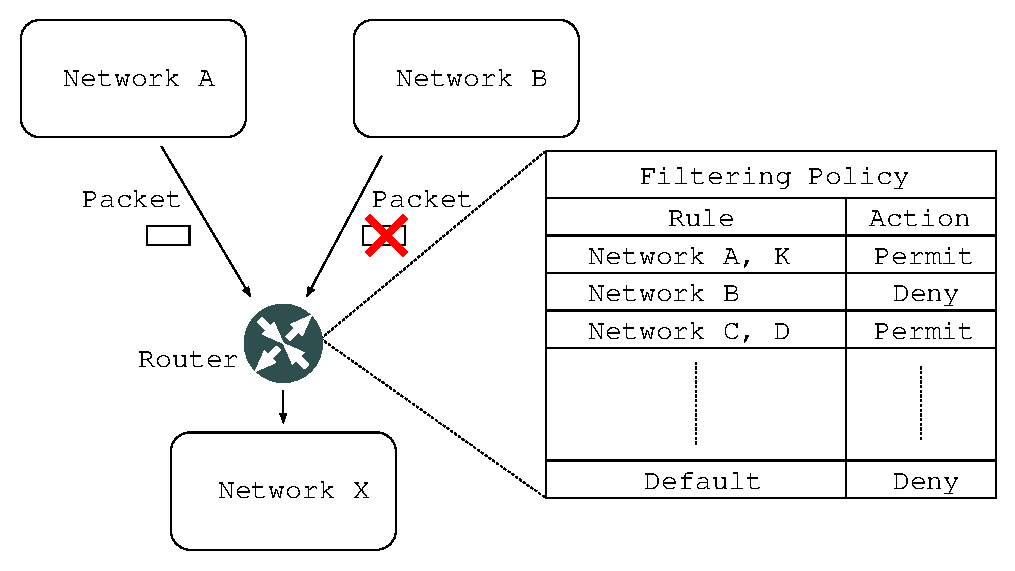
\includegraphics[scale=0.65]{filter-example.eps}
 }
\par
\vspace{5mm}
入ってくるパケットをポリシーに従ってルータで分類
\end{figure}
\end{frame}


%2枚目
\begin{frame}{パケットフィルタリングの方法}
\vspace{1mm}
\hspace{1mm} {\large \textbf{線型探索}} \hspace{48mm} {\large \textbf{その他}}
\vspace{2mm}
\begin{figure}
 \centering{
  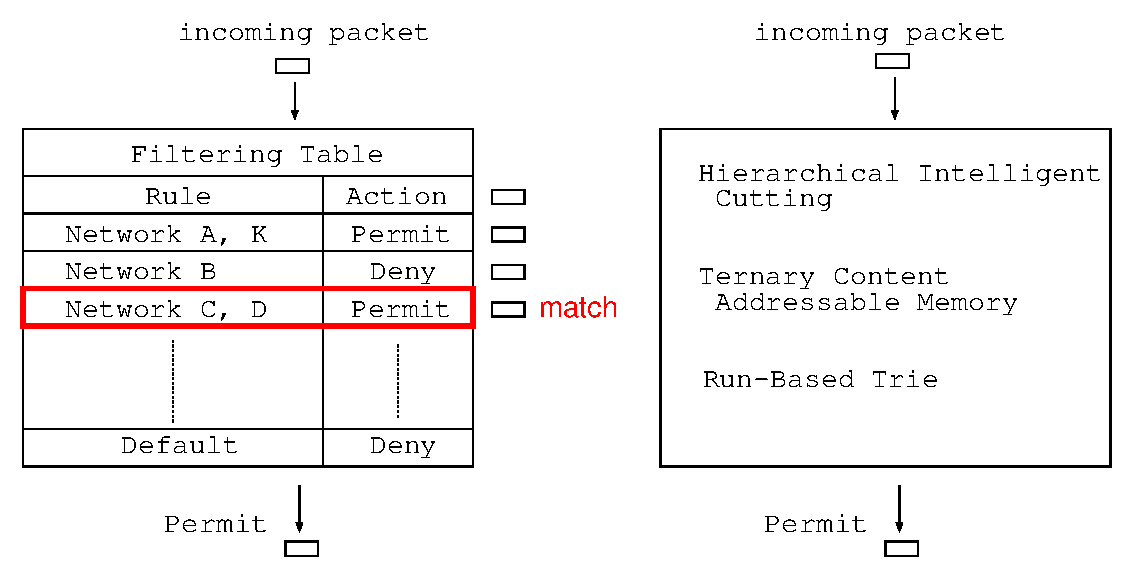
\includegraphics[scale=0.65]{filtering.eps}
 }
\end{figure}
\end{frame}


%3枚目
\begin{frame}{Run-Based Trie(三河,田中,$2011$)}

\vspace{1mm}
{\large \color{black}連の開始位置$i$ビット目ごとにトライ$T_{i}$を構成
}
\vspace{2mm}

\begin{figure}[h]
\begin{flushleft}
 \def\@captype{table}
 \begin{minipage}[t]{.38\textwidth}
  \begin{center}
  \begin{tabular}{ccc}
        & &    \\ \hline
 $Filter$ & & $F$ \\ \hline
 $R_{1}$ & & $0$ $*$ $1$ \\ 
 $R_{2}$ & & $*$ $0$ $0$ \\ 
 $R_{3}$ & & $1$ $1$ $0$ \\ 
 $R_{4}$ & & $1$ $1$ $*$ \\ 
 $R_{5}$ & & $0$ $*$ $*$ \\ 
 $R_{6}$ & & $*$ $1$ $*$ \\ \hline
  \end{tabular}
  \end{center}
 %\tblcaption{左側の表の見出し}
 %\label{左側の表へのラベル}
 \end{minipage}
 \hfill
 %
 \begin{minipage}[c]{.60\textwidth}
 %\caption{Run-Based Trie}
 \scalebox{0.7}{\input{rbtrie.tps}}
%\label{図へのラベル}
 \end{minipage}
\end{flushleft}
\end{figure}


\end{frame}


\begin{frame}{Simple Search でパケット $011$ を分類}
\vspace{3mm}

\begin{figure}[h]
\begin{center}
 \def\@captype{table}
 \begin{minipage}[t]{.48\textwidth}
  \begin{center}
  \begin{tabular}{ccc}
        & &    \\ \hline
 $Filter $& & $F$ \\ \hline
 \color{red}{$R_{1}$} & & {\color{red} $0$} $*$ $1$ \\ 
 $R_{2}$ & & $*$ $0$ $0$ \\ 
 $R_{3}$ & & $1$ $1$ $0$ \\ 
 $R_{4}$ & & $1$ $1$ $*$ \\ 
 {\color{red} $R_{5}$} & & {\color{red} $0$} $*$ $*$ \\ 
 $R_{6}$ & & $*$ $1$ $*$ \\ \hline
  \end{tabular}
  \end{center}
 %\tblcaption{左側の表の見出し}
 %\label{左側の表へのラベル}
 \end{minipage}
 \hfill
 %
 \begin{minipage}[c]{.40\textwidth}
 %\caption{Run-Based Trie}
 \scalebox{0.7}{\input{simple1.tps}}
%\label{図へのラベル}
 \end{minipage}
\end{center}
\end{figure}

\vspace{10mm}
\centering{
  \begin{tabular}{|c|c|c|c|c|c|c|} \hline
 最優先ルール & $R_{1}$ &  $R_{2}$ &  $R_{3}$ &  $R_{4}$ &  $R_{5}$ &  $R_{6}$ \\ \hline
 $-1$ $\rightarrow$ {\color{red} $5$} & $0$ $\rightarrow$ {\color{red} $1$} & $0$ & $0$ & $0$ & $0$ $\rightarrow$ {\color{red}$1$} & $0$ \\ \hline 
  \end{tabular}
%合致しているルール $\{ R_{5} \}$,現在の最優先ルール $R_{5}$
}
\end{frame}


\begin{frame}{Simple Search でパケット $011$ を分類}

\begin{figure}[h]
\begin{center}
 \def\@captype{table}
 \begin{minipage}[t]{.48\textwidth}
  \begin{center}
  \begin{tabular}{ccc}
        & &    \\ \hline
 $Filter $& & $F$ \\ \hline
 $R_{1}$ & & $0$ $*$ $1$ \\ 
 $R_{2}$ & & $*$ $0$ $0$ \\ 
 $R_{3}$ & & $1$ $1$ $0$ \\ 
 $R_{4}$ & & $1$ $1$ $*$ \\ 
 $R_{5}$ & & $0$ $*$ $*$ \\ 
 {\color{red} $R_{6}$} & & $*$ {\color{red} $1$} $*$ \\ \hline
  \end{tabular}
  \end{center}
 %\tblcaption{左側の表の見出し}
 %\label{左側の表へのラベル}
 \end{minipage}
 \hfill
 %
 \begin{minipage}[c]{.40\textwidth}
 %\caption{Run-Based Trie}
 \scalebox{0.7}{\input{simple2.tps}}
%\label{図へのラベル}
 \end{minipage}
\end{center}
\end{figure}

\vspace{10mm}
\centering{
  \begin{tabular}{|c|c|c|c|c|c|c|} \hline
 最優先ルール & $R_{1}$ &  $R_{2}$ &  $R_{3}$ &  $R_{4}$ &  $R_{5}$ &  $R_{6}$ \\ \hline
  $5$ & $1$ & $0$ & $0$ & $0$ & $1$ & $0$ $\rightarrow$ {\color{red}$1$} \\ \hline 
  \end{tabular}
%合致しているルール $\{ R_{5} \}$,現在の最優先ルール $R_{5}$
}

\end{frame}


\begin{frame}{Simple Search でパケット $011$ を分類}

\begin{figure}[h]
\begin{center}
 \def\@captype{table}
 \begin{minipage}[t]{.58\textwidth}
  \begin{center}
  \begin{tabular}{ccc}
        & &    \\ \hline
 $Filter $& & $F$ \\ \hline
 {\color{red} $R_{1}$} & & $0$ $*$ {\color{red} $1$} \\ 
 $R_{2}$ & & $*$ $0$ $0$ \\ 
 $R_{3}$ & & $1$ $1$ $0$ \\ 
 $R_{4}$ & & $1$ $1$ $*$ \\ 
 $R_{5}$ & & $0$ $*$ $*$ \\ 
 $R_{6}$ & & $*$ $1$ $*$ \\ \hline
  \end{tabular}
  \end{center}
 %\tblcaption{左側の表の見出し}
 %\label{左側の表へのラベル}
 \end{minipage}
 \hfill
 %
 \begin{minipage}[c]{.40\textwidth}
 %\caption{Run-Based Trie}
 \scalebox{0.7}{\input{simple3.tps}}
%\label{図へのラベル}
 \end{minipage}
\end{center}
\end{figure}

%\vspace{5mm}
\centering{
  \begin{tabular}{|c|c|c|c|c|c|c|} \hline
 最優先ルール & $R_{1}$ &  $R_{2}$ &  $R_{3}$ &  $R_{4}$ &  $R_{5}$ &  $R_{6}$ \\ \hline
 $5$ $\rightarrow$ {\color{red} $1$} & $1$ $\rightarrow$ ${\color{red} 2}$ & $0$ & $0$ & $0$ & $1$ & {\color{red}$1$} \\ \hline 
  \end{tabular}
%合致しているルール $\{ R_{5} \}$,現在の最優先ルール $R_{5}$
}

%\centering{
%合致しているルール $\{ R_{5}, \ R_{6}, \ R_{1} \}$,現在の最優先ルール $R_{1}$
%}

\vspace{5mm}

探索終了.パケット$011$に合致する最優先ルールは $R_{1}$
\end{frame}

\section{決定木を用いた Run-Based Trie の探索法}

\begin{frame}{集合族(Simple Searchでの$T_{i}$の辿り方の場合分け)}
\vspace{-3mm}
\centering{
 \scalebox{0.6}{\input{rbtrie.tps}}
}
\vspace{-2mm}
 \begin{align*}
  S_{1} &= \{\{ R_{1}^{1}, \ \underline{ R_{5}^{1}} \}, \ \{ \underline{ R_{4}^{1}} \}, \ \{\underline{ R_{3}^{1}}, \ \underline{ R_{4}^{1}} \}, \ \phi \}  \\
  S_{2} &= \{ \{ \underline{ R_{2}^{1}} \}, \ \{ \underline{ R_{6}^{1}} \}, \ \phi \}  \\
  S_{3} &= \{ \{ \underline{ R_{1}^{2}} \}, \ \phi \} 
 \end{align*}
集合族の直積$|S_{1}| \times |S_{2}| \times |S_{3}|$を取り,対応するルールを付与 \\ 
\vspace{1mm}
%$\rightarrow$ 
連の合致の組み合わせを全て列挙
\end{frame}

\begin{frame}{決定木}
%\vspace{10mm}
 \centering{
  \scalebox{0.8}{\input{dtree.tps}}
 }
 \par

\color{red}{Run-Based Trieに従って決定木を辿るだけで,パケットを分類可能}
 %\begin{flushleft}
 % 括弧中の{\color{red}赤い下線}が引かれた{\color{red}文字}は,$\phi$の為に展開されたもの
 %\end{flushleft}
\end{frame}

\begin{frame}{決定木によりパケット$011$を探索}
%\vspace{10mm}
 \centering{
  \scalebox{0.8}{\input{dtreenum.tps}}
 }
 \par

Run-Based Trie を用いて決定木を辿る.最優先ルールは $R_{1}$
 %\begin{flushleft}
 % 括弧中の{\color{red}赤い下線}が引かれた{\color{red}文字}は,$\phi$の為に展開されたもの
 %\end{flushleft}
\end{frame}


%11枚目
\begin{frame}{実験結果}
 \centering{
  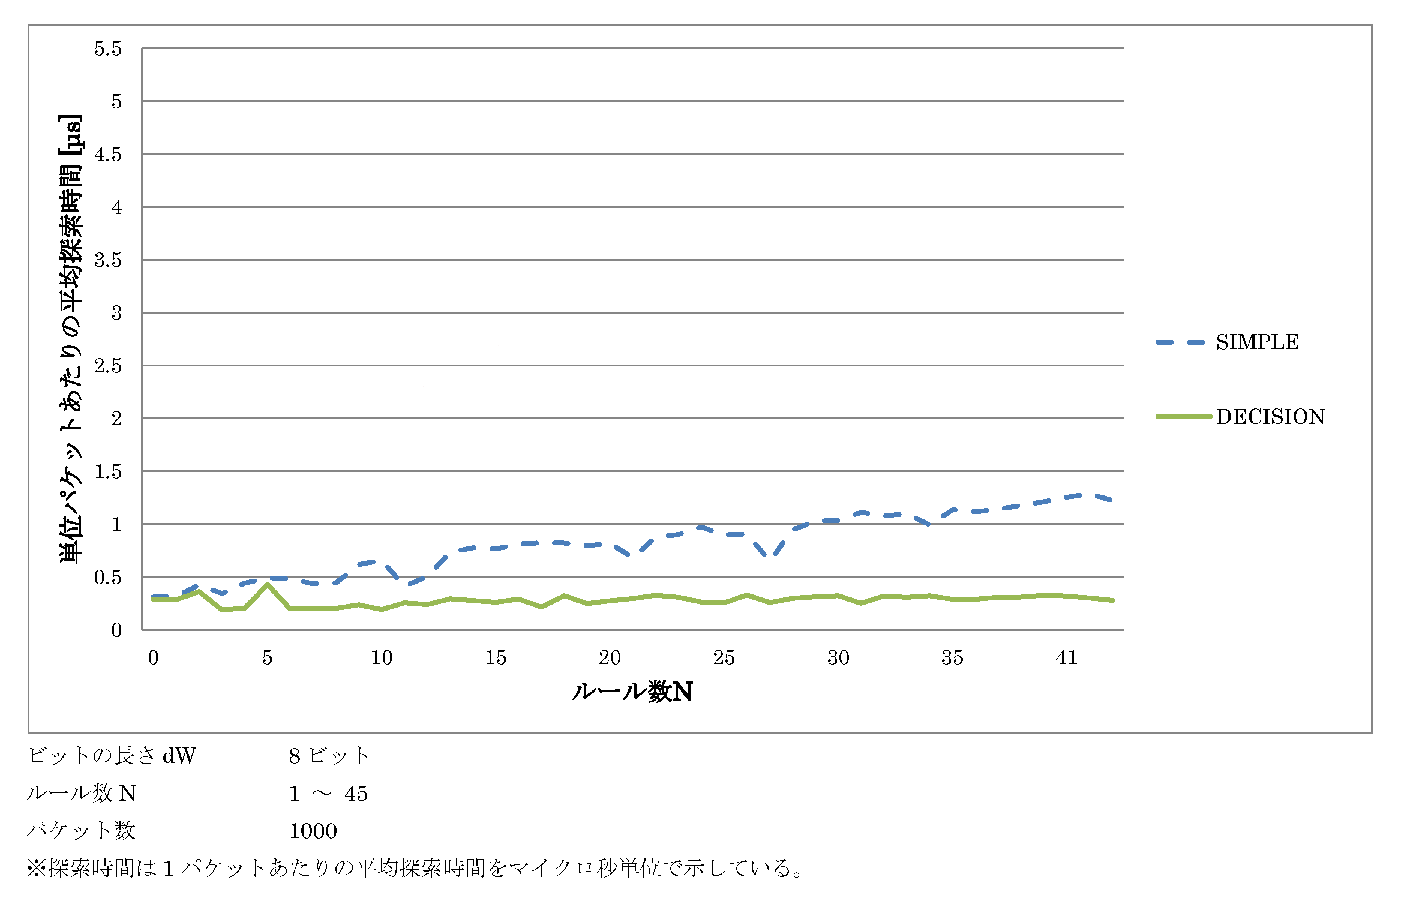
\includegraphics[scale=0.5]{result2.eps}
 }
  %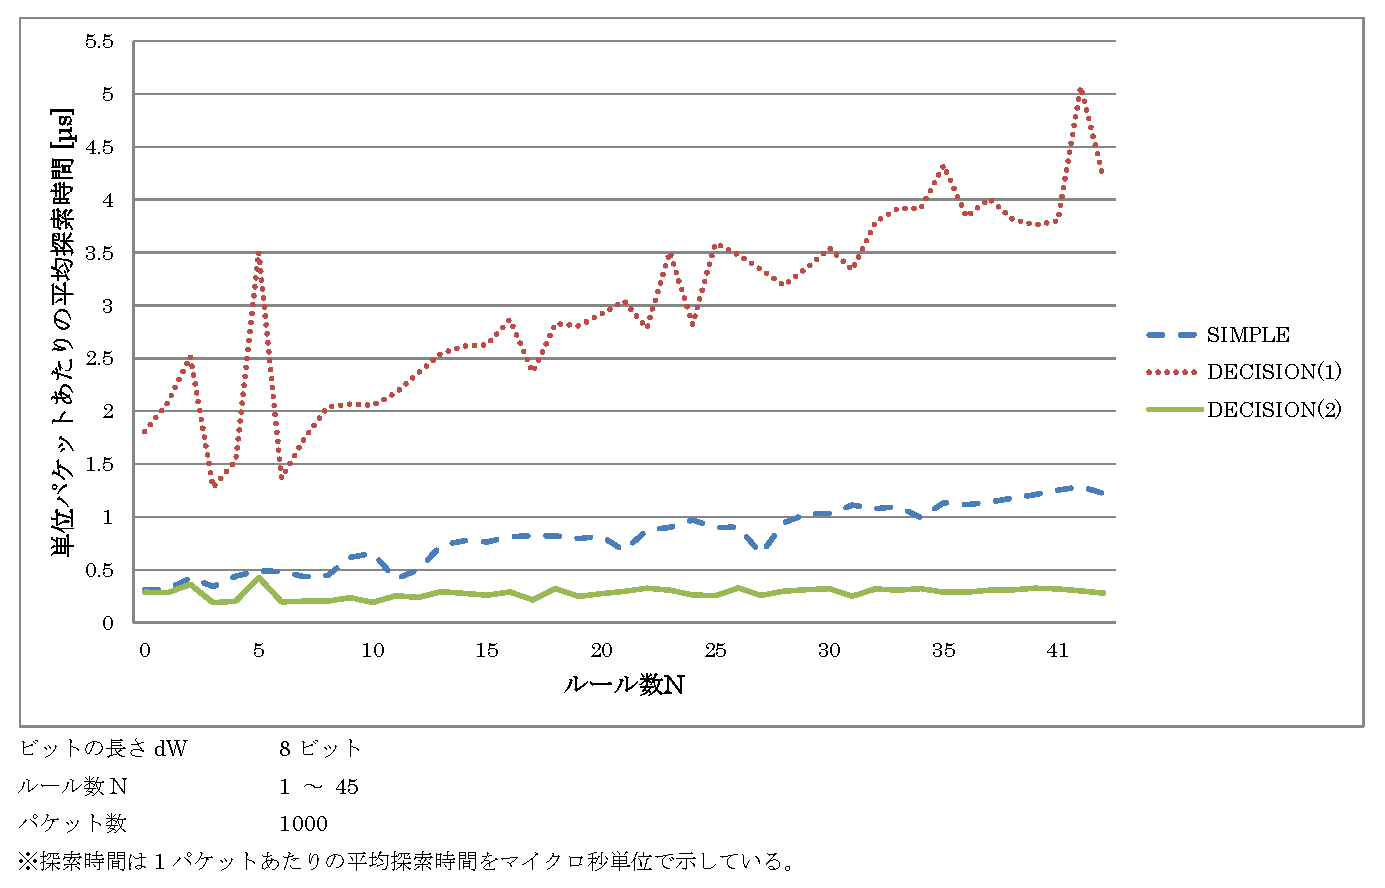
\includegraphics[scale=0.5]{kekka_fig_20121112-1-crop.eps}
\end{frame}


\section{まとめと今後の課題}
%12枚目
\begin{frame}{まとめと今後の課題}

\begin{center}
決定木を用いて Run-Based Trie を探索することにより,\\
\vspace{3mm}
フィルタリングルールの数$N$に依存せず探索
\end{center}

 \par
 \vspace{10mm}


 {\large 今後の課題}

 \vspace{3mm}
 \begin{itemize}
  \item Simple Searchの全ての辿り方を組み合わせるので,\\ 
決定木の空間計算量が膨大 $\rightarrow$ 枝刈りアルゴリズムが必要
  \vspace{3mm}
  \item 決定木の空間計算量の算出
  \vspace{3mm}
  \item プログラムを作成して,$16$ビット以上での実装実験
 \end{itemize}

\end{frame}

%
% \section*{references}
% \begin{frame}[allowframebreaks]{References}
%  \scriptsize
%  \bibliographystyle{jplain}
%  \bibliography{ebibtex}
% \end{frame}
 %
% \slide{ご清聴ありがとうございました.}
%
\end{document}
